\chapter{evaluation}\label{chapter:evaluation}

To evaluate the project researchers at both Imperial College London and Kings College London have been consulted for feedback. Since the evaluation group is relatively small (9 users), the interviews were focused on gaining personal insights, rather than trying to amass data that, due to the sample size, no statistical conclusions could be drawn from.

The feedback sessions took the form of a structured interview where features were demonstrated, discussed and then some more traditional questionnaire questions were asked. I found that the most useful feedback came from informally speaking to the researchers as it gave a more personal glimpse into their world than a questionnaire ever could. 

\section{Scan Simulation}
The feedback required for scan simulation was firstly to determine whether or not this would be a useful tool for the researchers. If it was, then the limitations of the current implementation needed to be found to guide the development. In particular are all the parameters usually present when setting up an MRI scan available and what other artefacts are there that would be useful to simulate?

The researchers were asked 'How useful is this feature for you?' and their responses are shown below in figure \ref{fig:graph_scansimulation_1}.

\begin{figure}[h]
    \centering
	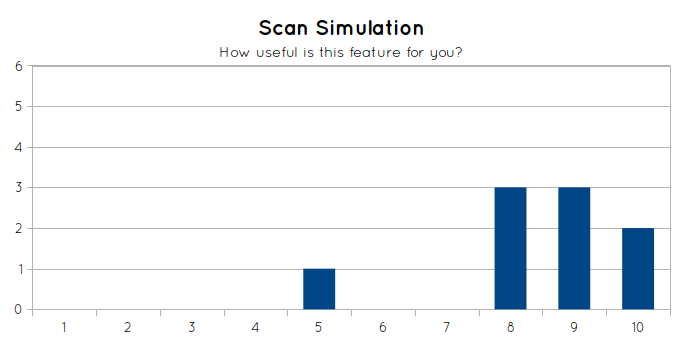
\includegraphics[width=0.6\textwidth]{images/evaluation/graph_scan_simulation_1.png}
    \caption{1 is useless. 10 is very useful.}\label{fig:graph_scansimulation_1}
\end{figure}

The majority of users thought that this feature would be of use for them. The one notable exception on the graph was due to concerns that the complexity of the simulation currently implemented is a far cry from that required. More on that shortly.

The users were then asked 'Does it include all of the parameters that you would expect?' and 'Is the simulation realistic enough?' to get an idea of what other features need to be implemented. Their responses are shown in figure \ref{fig:graph_scan_simulation23}.

\begin{figure}[H]
  \centering
  \begin{subfigure}[b]{0.5\textwidth}
    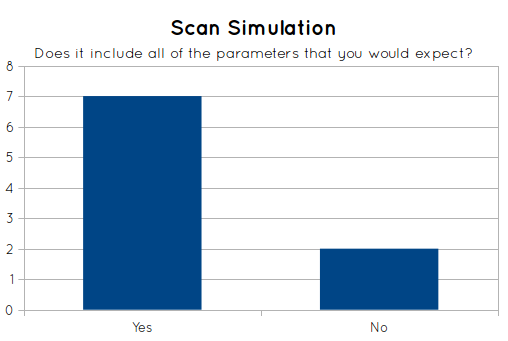
\includegraphics[width=\textwidth]{images/evaluation/graph_scan_simulation_2.png}
    %\caption{Variation 1}
    %\label{fig:graph_scansimulation_2}
  \end{subfigure}%
  ~ %add desired spacing between images, e. g. ~, \quad, \qquad, \hfill etc.
    %(or a blank line to force the subfigure onto a new line)
  \begin{subfigure}[b]{0.5\textwidth}
    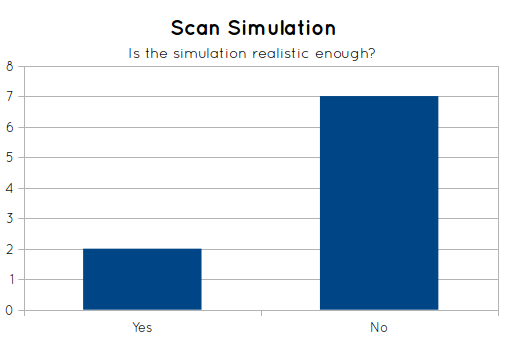
\includegraphics[width=\textwidth]{images/evaluation/graph_scan_simulation_3.png}
    %\caption{Variation 2}
    %\label{fig:graph_scansimulation_3}
  \end{subfigure}
  \caption{Responses to realism questions.}\label{fig:graph_scan_simulation23}
\end{figure}

For the most part the researchers felt that the control they have over the scan configuration was enough. One suggested that instead of specifying the value in pixels, which was a natural unit to use when dealing with a reconstructed volume, it would be good to have the option to specify mm instead, which more closely matches a MRI scanner. 

Another suggestion was the ability to specify a scan by selecting the two endpoints. This would give the user finer directional control and the ability to more easily specify shorter scans.

The question about the realism required of the simulation prompted the largest response. Quickly the feature list for potential improvements grew. As a reminder the only artefact currently implemented is a simple rotation which takes effect in between scanning slices.

\begin{itemize}
  \item \textbf{Additional movement artefacts.} Movement during an MRI scan does not manifest itself as blur, like many other imaging techniques. Instead a number of different artefacts occur including replication, where multiple copies of the object appear, or shadowing where objects in motion appears darker than their surroudings.

  \item \textbf{Translation + Enhanced Rotation}. Translations can be added alongside the rotations but there are also more fundamental changes that can be made to model the movement more realistically. Currently a uniform random variable decides the random rotation and this is unlikely to match the genuine movement of a fetus. For example a fetus is far more likely to nod than shake it's head. Data on fetal movement has been collected at different stages of development previously to establish behavioural patterns\cite{fetalmovement} and so this data could be repurposed to sample movements from a more representative distribution.

  \item \textbf{Interleaved acquisition.} Currently neighbouring slices in the simulated scan are acquired sequentially however in reality the order the slices are acquired is often interleaved (e.g. 1, 5, 10, ..., 2, 6, 11, ...). This is because the frequency of radio wave used to acquire a single slice isn't perfect and so when one slice is excited, slices adjacent to it are often excited as well, albeit to a lesser extent\cite{basicsofmri}. Scanning in an interleaved manner allows these adjacent slices time to relax before they are acquired. The upshot of this is that neighbouring slices are likely to be acquired further apart in time than those in the interleaved set. When simulating movement this sequence can be taken into account to match this.

  \item \textbf{Bias/Inhomogeneity.} The proximity of the fetus from the receiver coil can also have an effect on the scan. This can often create what is known as a bias or inhomogeneity which effectively results in areas of the scan being darker than they should be.

  \item \textbf{Noise.} The signal to noise ratio (SNR) plays an important role in deciding what resolution to scan at. Too high and the image will be too noisy, but too low and the image will be too blurry. Interestingly the noise that appears in MRI scans is not gaussian, but rician. This is because the image is acquired in the frequency domain (known as k-space) and this information is transformed to build an image space representation. Since the noise is gaussian in the frequency domain it becomes rician in the spatial domain.
  
  \item \textbf{Extend to Moving/Periodic Scans.} The way that a cine (moving MRI image) is acquired differs from the imaging of a static object. For periodic motion, like the beating of the heart, a number of scans are acquired and then those that happen to be at the same point in the cycle are used to reconstruct one frame in the animation. This is another area that could potentially be simulated.
\end{itemize}

These potential extensions raise the question of how much realism is required to effectively test reconstruction algorithms? Highly realistic MRI simulation has been done before and tools, such as MRiLab\cite{mrilab}, allow the user to experiment with different scan sequences, coils and more. However, how far along this path we need to go to test reconstruction algorithm remains an area where more research is needed.

\newpage
\section{Reconstruction}
The purpose of this part of the plugin was to get an idea of how researchers feel about manually labelling slice stacks to improve the quality of the reconstruction. 

When asked 'How important is it for you to manually guide the reconstruction process?' the majority preferred to have some degree of control over it. See figure \ref{fig:reconstructionguiding}. Those who were less concerned about this either weren't involved in the reconstruction process (and put 1) or felt that they do like the ability to guide it but would greatly prefer if it were automated.

\begin{figure}[h]
    \centering
  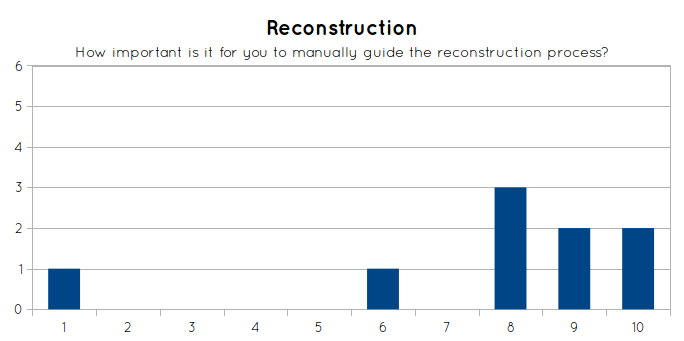
\includegraphics[width=0.6\textwidth]{images/evaluation/graph_reconstruction_1.png}
    \caption{1 is not at all. 10 is very important.}\label{fig:graph_reconstruction_1}
\end{figure}

When asked 'How likely are you to manually label stack sets to improve the reconstruction?' the responses were more varied. See figure \ref{fig:graph_reconstruction_2}. Most participants were willing to label slice stacks but there was more negativity towards this than before, and the impression received was that they do it begrudgingly.

Anecdotally it seems to take around 30 minutes to perform the pre-processing required for a single reconstruction. This involves manually inspecting each slice to gauge the quality, building a mask to specify the area to reconstruct and optionally adding landmarks to each stack.

Currently four landmarks can be used to aid the registration: both eyes and two points on the brain stem. In some cases, where the input data is good, this is not necessary, however if there is a large amount of movement then manual intervention is required.

When asked 'How long would you be willing to spend labelling landmarks for a reconstruction?' nobody was willing to spend more than 30 minutes and the majority would prefer it to take 10 minutes or below. See figure \ref{fig:graph_reconstruction_3}. It's difficult to say whether there may be some degree of "asking for more than you expect to get" going on but the consensus is that the time quickly adds up. It's fine if you have one reconstruction to do but when you come to large user studies with potentially hundreds of scans it simply doesn't scale.

\begin{figure}[H]
  \centering
  \begin{subfigure}[b]{0.5\textwidth}
    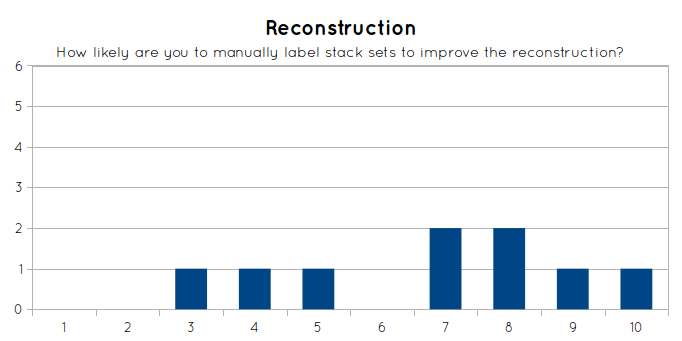
\includegraphics[width=\textwidth]{images/evaluation/graph_reconstruction_2.png}
    \caption{1 is no chance, 10 is very likely.}
    \label{fig:graph_reconstruction_2}
  \end{subfigure}%
  ~ %add desired spacing between images, e. g. ~, \quad, \qquad, \hfill etc.
    %(or a blank line to force the subfigure onto a new line)
  \begin{subfigure}[b]{0.5\textwidth}
    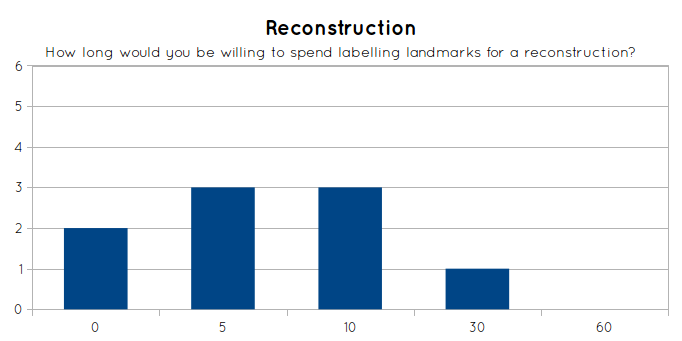
\includegraphics[width=\textwidth]{images/evaluation/graph_reconstruction_3.png}
    \caption{Time (minutes).}
    \label{fig:graph_reconstruction_3}
  \end{subfigure}
  \caption{}\label{fig:graph_reconstruction23}
\end{figure}

The plugin includes a simple tool that allows 13 landmarks to be specified on each slice stack before reconstruction. This was implemented with the view of trying to estimate how long the landmarking stage takes to perform. Constraints on how long I had to spend with each user on the evaluation, and also the level of familiarity of each user with the developing brain mean that the estimations here are quite rough, but do set the scene.

5 users were familiar enough with the brain to take part in the time trial (others specialise in other parts of the body). The stack being annotated had been simulated with up to 5 degrees of motion corruption but other than that was very clean and so there is little ambiguity finding the points. The times are shown in figure \ref{fig:landmarktimes}. 

\begin{figure}[h]
    \centering
  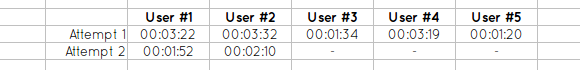
\includegraphics[width=0.8\textwidth]{images/evaluation/graph_reconstruction_landmark_times.png}
    \caption{There is large variance, but around 2 minutes seems reasonable.}\label{fig:landmarktimes}
\end{figure}

Taking these results with a pinch of salt it seems that around 10 seconds per landmark is a reasonable estimate for labelling of images, once the user is up to speed. With a large number of stacks per reconstruction and a large number of reconstructions in a study this soon adds up.

Another source of inefficiency comes from the use of a number of different pieces of software in the reconstruction process, which causes time to be wasted exporting and importing between them all. Integrating the entire process into one application should help reduce this penalty significantly.

My time spent with researchers indicated that overall they are willing to spend time labelling slice stacks, but only if they really need to, and only the minimum number required. Four landmarks is sufficient to define a rigid transformation (translation and rotation only) and this may prove sufficient for some scans. The more deformable the organ, however, the greater the number of landmarks required. The position of the landmarks is also important, having four landmarks along the same axis is of no use, and how likely the landmark is to be obscured is also a consideration.

One way to improve the efficiency of the landmarking step is to introduce the idea of iterated reconstruction. An initial reconstruction can be performed and then the user can be prompted to provide landmarks in areas of high uncertainty.

This procedure can then be iterated, with only small parts of the volume requiring reconstruction at each step, until the uncertainty is at an acceptable level.

If the iteration could also output the algorithm's current best guess for the user to tweak this would also save time. Moving the landmarking process from a completely manual "find all these landmarks" to more of a supervised "here are some landmarks - are they correct" approach will not only speed up the landmarking, but be less tedious for the user.

One problem that had not been anticipated were ambiguities determining which direction is left and which is right when placing landmarks. This is one of the limitations of DICOM, one of the most common medical image formats in use, and so some way of letting the user mark this, before a mask is created, would be useful.

The researchers still want a way to manually inspect the slices stacks to check their quality, either to establish why a reconstruction failed, or as a preliminary check. One feature that would help with this is the ability to view stacks side by side and scroll through them simultaneously.

Another point raised was that there is sometimes ambiguity when deciding what part of a landmark to mark. Having an example image of each landmark would clarify both what the user is looking for, and also where to mark it.

\newpage
\section{Visualization}
Three things. Understand. Clear. Configurable.

% General Format -> What we wanted to find out. Go through each question. For those that are quantitative give us a graph. For those that aren't then talk about What they said.